These are working notes for the low density parameters in {\tt MAESTRO}.

\section{Computing the Cutoff Values}

At several points in the algorithm, we compute {\tt anelastic\_cutoff\_coord}, 
{\tt base\_cutoff\_density\_coord}, and {\tt burning\_cutoff\_density\_coord} by 
setting the corresponding coordinate equal to $r$ as soon as $\rho_0(r)$ is less than 
or equal to that particular cutoff value (see Figure \ref{Fig:Cutoff}.
We compute the cutoff coordinate at the
coarsest level, and then set the coordinate at the next finer level to be twice that
of the coarser level.  We set the coordinates at the following points in the code:
%%%%%%%%%%%%%%%%%%%%%%%%%%%%%%%%%
\begin{figure}[hpb]
\centering
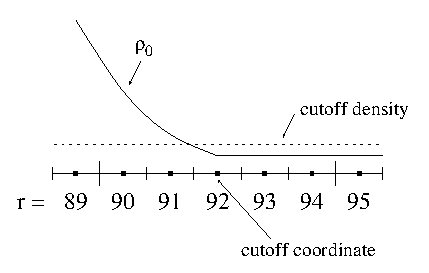
\includegraphics[width=4.0in]{\lodensfigpath/cutoff}\hspace{0.2in}
\begin{minipage}[b]{5.0in}
\caption[Relation between cutoff density and cutoff coordinates]
{Image of how the cutoff density and cutoff coordinates
are related.  This is drawn assuming {\tt drdxfac}=5.\vspace{2em}}
\end{minipage}
\label{Fig:Cutoff}
\end{figure}
%%%%%%%%%%%%%%%%%%%%%%%%%%%%%%%%%

\begin{itemize}

\item After we call {\tt initialize} in {\tt varden}.

\item At the beginning of {\tt advance\_timestep}.

\item After each call to {\tt advect\_base\_dens}.

\item After we ``{\tt correct base}'' (by setting $\rho_0 = \overline{\rho}$ in
  plane-parallel and $\rho_0 = \rho_0 + {\bf{Avg}}(\rho - \rho_0)$ in spherical).

\item At the beginning of the second-half of the algorithm (Step 6), we reset
  the coordinates to the base-time values using $\rho_0^n$.

\end{itemize}

\section{Density vs. Coordinate}

Note that saying $r\ge$ {\tt anelastic\_cutoff\_coord} is analogous to saying $\rho_0(r)\le$ {\tt anelastic\_cutoff}.  Also, saying $r<$ {\tt anelastic\_cutoff\_coord} is analogous to saying $\rho_0(r)>$ {\tt anelastic\_cutoff}.  Ditto for {\tt base\_cutoff\_density} and {\tt base\_cutoff\_density\_coord}.

\section{anelastic\_cutoff}\label{Sec:Anelastic Cutoff}

The {\tt anelastic\_cutoff} is the density below which we modify the constraint.


\begin{itemize}

\item In {\tt probin}, {\tt anelastic\_cutoff} is set to $3\times 10^6$ by default.

\item In {\tt init\_base\_state}, we give a warning if {\tt anelastic\_cutoff}
  is smaller than the minimum model density.  Then, if ${\tt anelastic\_cutoff} 
  < {\tt base\_cutoff\_density}$, we abort the program.

\item In {\tt make\_div\_coeff}, for 
  $r \ge {\tt anelastic\_cutoff\_coord}$, we set
  ${\tt div\_coeff}(n,r) = {\tt div\_coeff}(n,r-1) * \rho_0(n,r)/\rho_0(n,r-1)$.

\item in {\tt make\_S}, we set {\tt delta\_gamma1\_term} and {\tt delta\_gamma1} 
  to zero for $r \ge {\tt anelastic\_cutoff\_coord}$.

\item In {\tt sponge}, {\tt anelastic\_cutoff} is used in a problem
  dependent way.

\end{itemize}

\section{base\_cutoff\_density}\label{Sec:Base Cutoff Density}

The {\tt base\_cutoff\_density} is the lowest density that we model.

\begin{itemize}

\item In {\tt probin}, {\tt base\_cutoff\_density} is set to $3\times 10^6$ by default.

\item In {\tt init\_base\_state}, we give a warning of {\tt base\_cutoff\_density}
  is smaller than the minimum model density.  Then, if ${\tt anelastic\_cutoff} 
  < {\tt base\_cutoff\_density}$ we abort the program.

\item In {\tt base\_state}, we compute a physical cutoff location,
  {\tt base\_cutoff\_density\_loc}, which is defined as the physical
  location of the first cell-center at the coarsest level for which
  $\rho_0 \le {\tt base\_cutoff\_density}$.  This is a trick used for making
  the data consistent for multiple level problems.  When we are generating the 
  initial background/base state, if we are above {\tt base\_cutoff\_density\_loc}, 
  just use the values for $\rho,T$, and $p$ at {\tt base\_cutoff\_density\_loc}.
  When we check whether we are in HSE, we use {\tt base\_cutoff\_density\_loc}.

\item In {\tt make\_hgrhs}, {\tt make\_macrhs}, and {\tt make\_w0}, 
  we only add the volume discrepancy for $r < {\tt base\_cutoff\_density\_coord}$
  (in plane parallel) and if $\rho_0^{\rm cart} > {\tt base\_cutoff\_density}$ 
  (in spherical).

\item In {\tt mkrhohforce} for plane-parallel, for
  $r \ge {\tt base\_cutoff\_density\_coord}$, we
  compute $\nabla p_0$ with a difference stencil instead of simply
  setting it to $\rho_0 g$.

\item In {\tt update\_scal}, if $\rho \le {\tt base\_cutoff\_density}$
   and {\tt do\_eos\_h\_above\_cutoff}, we call the EOS to compute $h$.

\item In {\tt update\_scal}, if $\rho \le {\tt base\_cutoff\_density}/2$
   we set it to ${\tt base\_cutoff\_density}/2$.

\item In {\tt make\_grav} for spherical, we only add the enclosed mass if
  $\rho_0 > {\tt base\_cutoff\_density}$.

\item In {\tt enforce\_HSE}, we set $p_0(r+1) = p_0(r)$ for 
  $r \ge {\tt base\_cutoff\_density\_coord}$.

\item In {\tt make\_psi} for plane-parallel, we only compute $\psi$ for 
  $r < {\tt base\_cutoff\_density\_coord}$.

\end{itemize}

\section{burning\_cutoff}

The burning cutoff determines where we call the reaction network to
get the nuclear energy generation rate and composition changes.  For
densities below the burning cutoff, we do not call the network.

\begin{itemize}

\item In {\tt probin}, {\tt burning\_cutoff\_density} is set to 
  {\tt base\_cutoff\_density}.  There is no option to set 
  {\tt burning\_cutoff\_density} using the inputs file.

\item In {\tt react\_state}, we only call the burner if 
  $\rho >$ {\tt burning\_cutoff\_density}.


\end{itemize}


\section{buoyancy\_cutoff\_factor}

The {\tt buoyancy\_cutoff\_factor} is used to zero out the forcing terms
to the velocity equation at low densities.

\begin{itemize}

\item In {\tt init\_base\_state} we print out the value of the
   the density at which the buoyancy cutoff would take effect,
   {\tt buoyancy\_cutoff\_factor * base\_cutoff\_density}.

\item In {\tt mk\_vel\_force}, we zero out {\tt rhopert}, the
   perturbational density used in computing the buoyancy force,
   if $\rho < \mathtt{buoyancy\_cutoff\_factor * base\_cutoff\_density}$.

\item In {\tt mk\_vel\_force}, for spherical problems, we 
   zero out {\tt centrifugal\_term}, the centrifugal force for
   rotating stars, if $\rho < \mathtt{buoyancy\_cutoff\_factor *
   base\_cutoff\_density}$.

\end{itemize}





